\section{Convex Hull}\label{sec:ch}
We next consider the \textit{convex hull
score}.  We briefly recall the definition of a convex set and then
define this score function.


\begin{definition}
	A set in a metric space is \textbf{convex} if the shortest geodesic segment between any two points in the set is entirely 
	contained within that set.
\end{definition}



\begin{figure}[h]
	\centering
	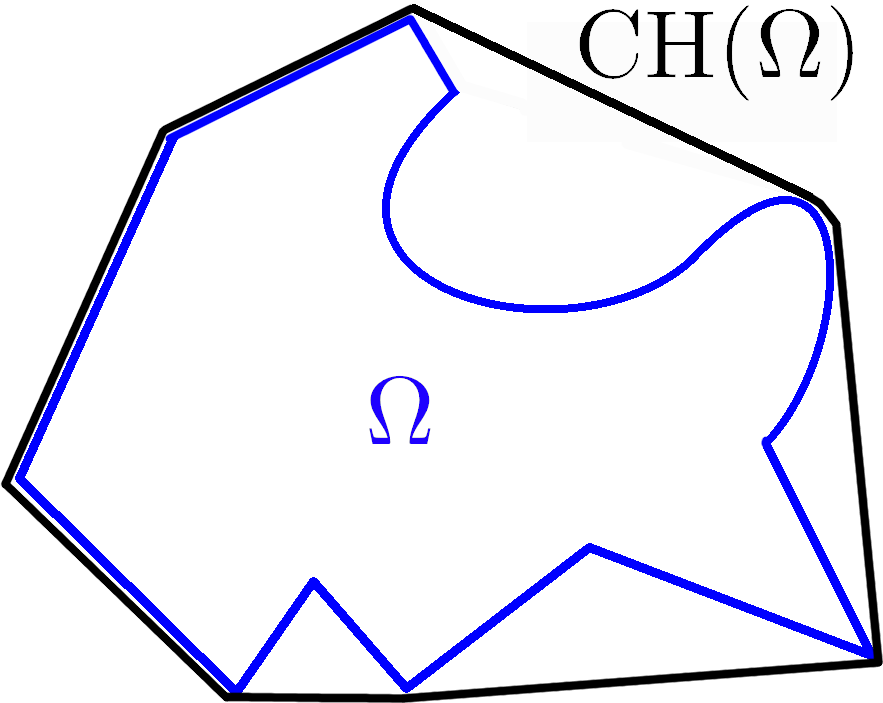
\includegraphics[width=.5\textwidth]{figs/ch_example.png}
	\caption{A region $\Omega$ and its convex hull.}
	\label{fig:ch_example}
\end{figure}

\begin{definition}
  Let $\mathrm{conv}(\Omega)$ denote the \textit{convex hull} of
  a region $\Omega$ in either the sphere or the plane, which is the
  smallest convex region containing $\Omega$.  Then we define the
  \textit{convex hull score} of $\Omega$ as 
  \begin{align*}
    \mathrm{CH}(\Omega)=
    \frac{\mathrm{area}(\Omega)}{\mathrm{area}(\mathrm{conv}(\Omega))}
  \end{align*}
\end{definition}



Throughout this section, let $\vphi:\Omega \to \R^2$ be a 
map projection defined on a patch of the sphere $\Omega\subset \mbb{S}^2$.


We begin by observing that such a projection must preserve certain geometric properties within these patches.
\begin{lemma}~\label{lem:CH_prep}
	If $\vphi$ preserves the ordering of regions induced by their convex hull scores, then the following must 
	hold:
	\begin{enumerate}
		\item $\vphi$ and $\vphi^{-1}$ send convex regions to convex regions
		\item $\vphi$ sends every segment of a great circle on the sphere to a line segment in the plane.  That is, it preserves geodesics.
		\item There exists a region $U$ in our patch
		such that for any regions $A,B\subset U$, if 
		$A$ and $B$ have equal area on the sphere, then 
		$\vphi(A)$ and $\vphi(B)$ have equal area in the plane.  The same holds 
		for $\vphi^{-1}$ for all pairs of regions inside of $\vphi(U)$.
	\end{enumerate}
\end{lemma}

\begin{figure}[h]
	\centering
	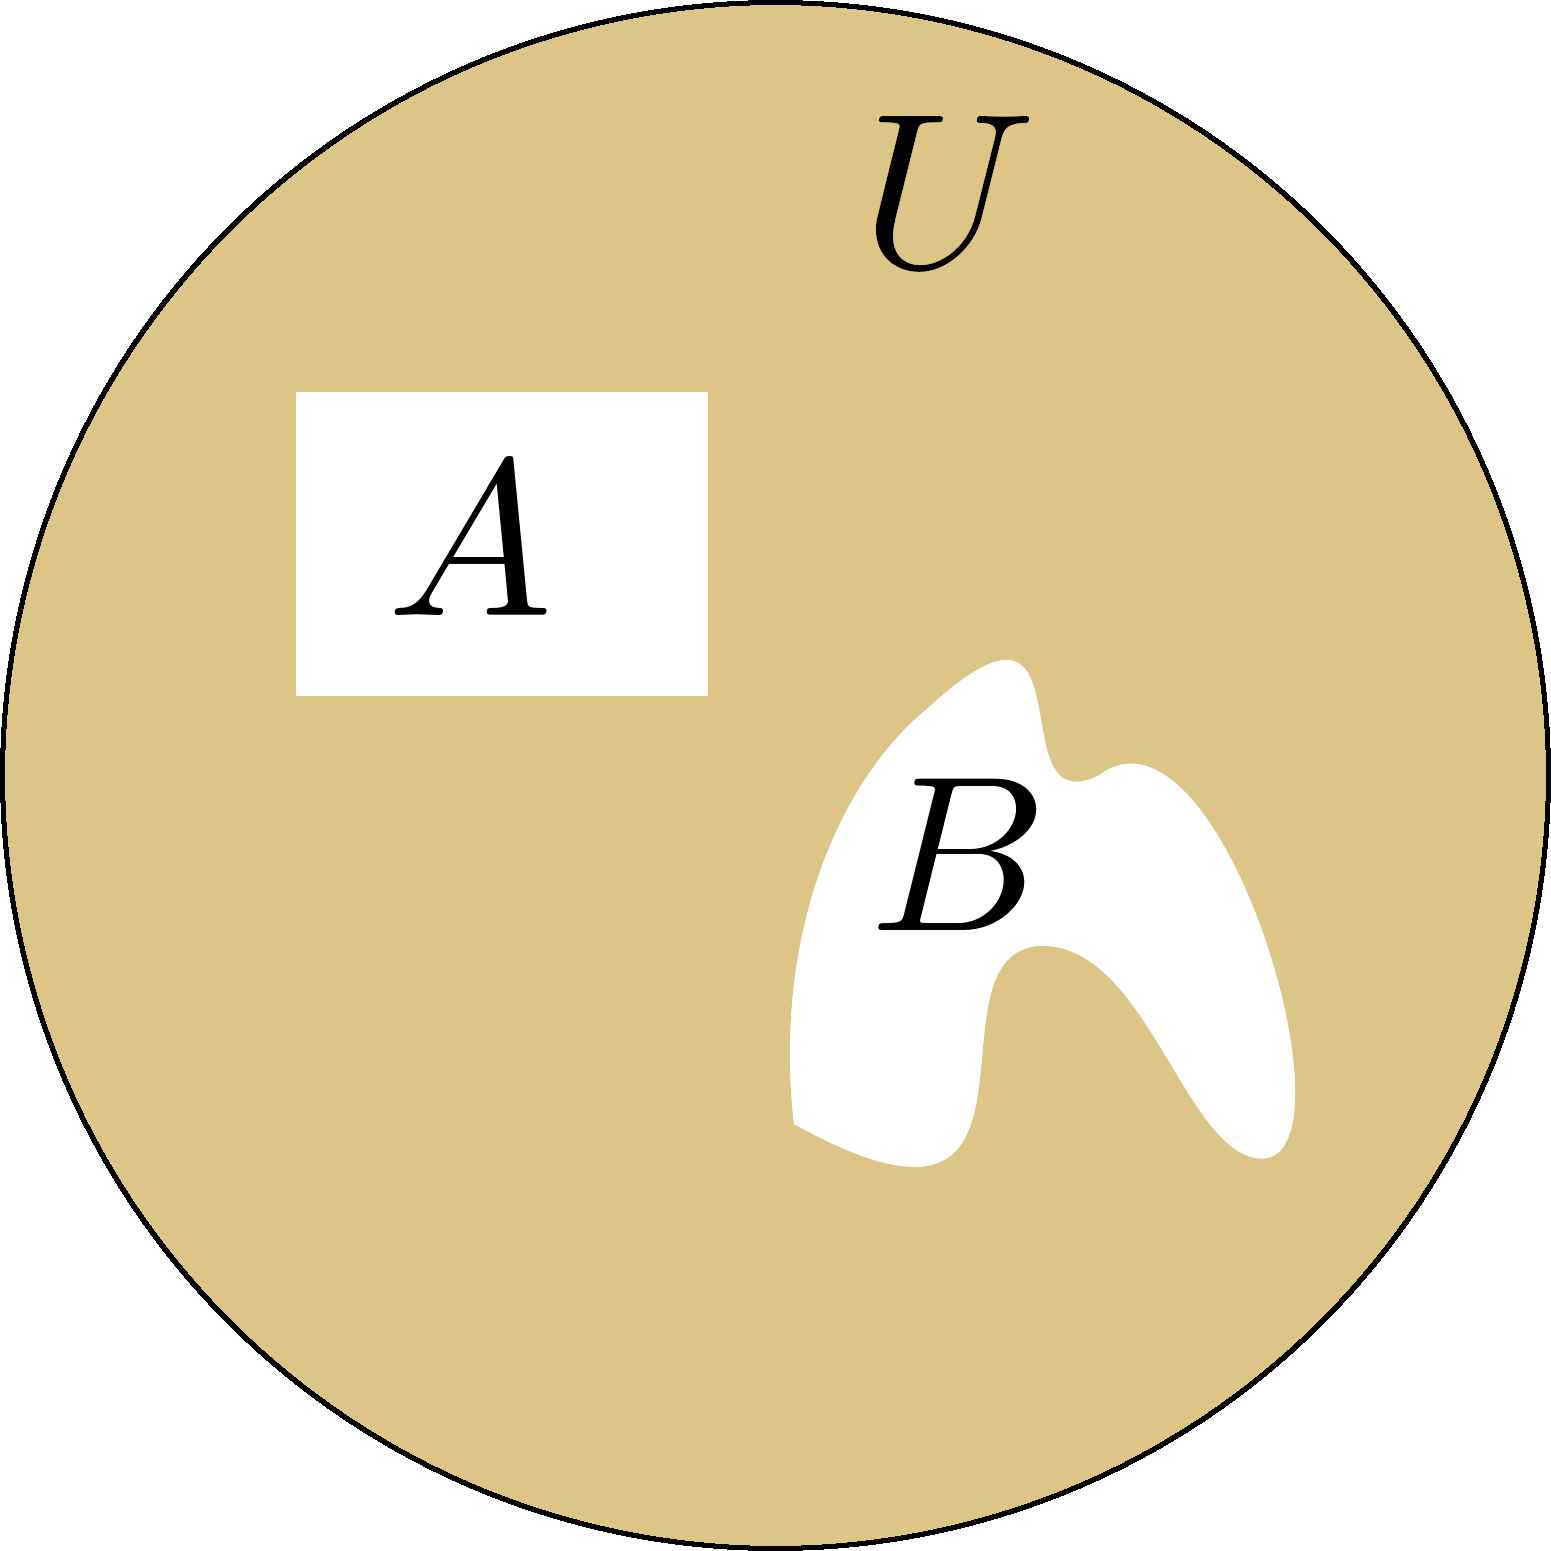
\includegraphics[width=.25\textwidth]{figs/ch_sphere_schema.png}
	\caption{Two equal area regions $A$ and $B$ removed from $U$.}
	\label{fig:ch_schema}
\end{figure}



\begin{proof}
	\ \\
	
	\vspace*{-2em}
	\begin{enumerate}
		\item[] The proof of (1) follows from the idea that any projection which preserves the convex hull score ordering of regions must 
		preserve the maximizers in that ordering.   Here, the maximizers are convex sets.
		
		\item[]  Suppose, for the sake of contradiction, that there is some geodesic segment $s$ on the sphere such that $\vphi(s)$ is not a line segment. Take $s$ and 
		consider its $\eps$-thickening, which is the region defined by the union of $\eps$ caps centered at each point 
		along the segment.  We can observe that since $\vphi(s)$ is not a line segment, there is some small $\delta$ such that the $\delta$-thickening of $\vphi(s)$ is not convex.  
		
		The $\eps$-thickening of $s$ is convex for all $\eps$, so by (1), $\vphi$ will send this to a convex region.  However, there must be some $\eps'$ such that the $\eps'$-thickening of $s$ is sent to the $\delta$-thickening of $\vphi(s)$, which contradicts the fact that the image of these thickenings are convex.
		
		The proof that $\vphi^{-1}$ sends line segments in the plane to great circle segments on the sphere is analogous.  
		
		This proves (2).
		
		
		
\item[] To show (3), let our region $U\subset\Omega$ be a cap, without loss of generality.  Take $A,B$ to be regions of equal area such that $A$ and $B$ are properly contained in the interior of $U$, as in \Cref{fig:ch_schema}.  Define two new regions $X=U\ssm A$ and $Y=U\ssm B$, i.e. these regions are equal to $U$ with $A$ or $B$ deleted, respectively.  

The cap $U$ is itself the convex hull of both $X$ and $Y$, and since $A$ and $B$ have equal area, we have that $\mathrm{CH}(X) = \mathrm{CH}(Y)$.  Since $U$ is a cap, it is convex, so by (1), $\vphi(U)$ is also convex.  Since $\vphi$ preserves the ordering of convex hull scores and $X$ and $Y$ had equal scores on the sphere, $\vphi$ must send $X$ and $Y$ to regions in the plane which also have the same convex hull score.  Furthermore, the convex hulls of $\vphi(X)$ and $\vphi(Y)$ are $\vphi(U)$.

We can then write 
\begin{align*}
\mathrm{CH}(X) &= \mathrm{CH}(Y)\\
\ &\\
\frac{\mathrm{Area}(\vphi(X))}{\mathrm{Area}(\vphi(U))} &= \frac{\mathrm{Area}(\vphi(Y))}{\mathrm{Area}(\vphi(U))}\\
\ &\\
\frac{\mathrm{Area}(\vphi(U)) - \mathrm{Area}(\vphi(A))}{\mathrm{Area}(\vphi(U))} &= \frac{\mathrm{Area}(\vphi(U)) - \mathrm{Area}(\vphi(B))}{\mathrm{Area}(\vphi(U))}\\
\ &\\
\mathrm{Area}(\vphi(A)) &= \mathrm{Area}(\vphi(B))
\end{align*}
 which is what we wanted to show.  The proof that $\vphi^{-1}$ also has this property is analogous.  This proves (3).
\end{enumerate}
\end{proof}

We can now show that no map projection can preserve the convex hull score ordering of regions by proving that there is no projection from a patch on the sphere to the plane which has all three of the properties described above in \Cref{lem:CH_prep}. 


\begin{theorem}
	There does not exist a map projection satisfying the 
	conditions in Lemma~\ref{lem:CH_prep}
\end{theorem}
\begin{proof}
	Assume that such a map, $\vphi$, exists, and restrict 
	it to $U$ as above. Let $T\subset U$ be a 
	spherical equilateral triangle with 
	$\mathrm{Diam}(T)<\frac{\mathrm{Diam}(U)}{3}$, centered at 
	the center of $U$. Let $T_1$ and $T_2$ be two 
	congruent triangles meeting at a point and 
	each sharing a face with $T$, as in \Cref{fig:sphtris}.

\begin{figure}[h]
	\centering
	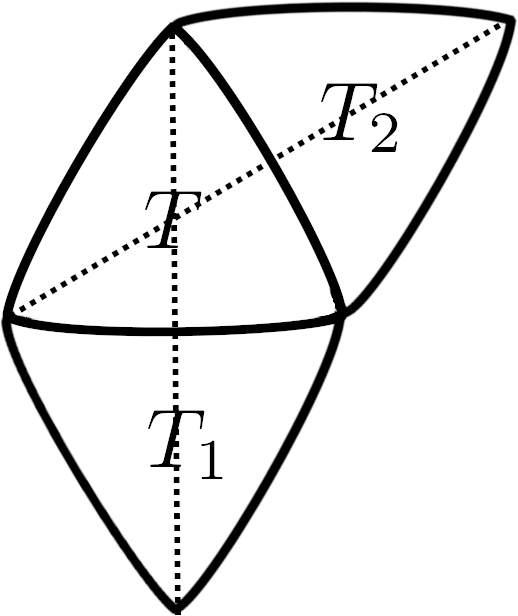
\includegraphics[width=.25\textwidth]{figs/spheretri.png}
	\caption{The spherical regions $T,T_1,T_2$.}
	\label{fig:sphtris}
\end{figure}












We first argue that the images of $T\cup T_1$ and $T\cup T_2$ are parallelograms.

Without loss of generality, consider. $T\cup T_1$.  By construction, it is a 
convex spherical quadrilateral. By symmetry, its geodesic 
diagonals on the sphere divide it into four triangles of equal area, since the long diagonal splits $T$ and $T_1$ in 
half, and $T$ and $T_1$ have the same area.


		Since $\vphi$ sends spherical geodesics to line segments in the plane, it must send 
		$T\cup T_1$ to a Euclidean quadrilateral $Q$ whose diagonals 
		are the images of the diagonals of the spherical quadrilateral $T\cup T_1$.
		
		 Since 
		$\vphi$ sends equal area regions to equal area 
		regions, it follows that the diagonals 
		of $Q$ split it into four equal area triangles.
		
		We now argue that this implies that $Q$ is a Euclidean parallelogram by showing that its diagonals bisect each other.  Since the four triangles 
		formed by the diagonals of $Q$ are all the same area, we can pick two of these triangles which share a side 
		and consider the larger triangle formed by their union.  One side of this triangle is a diagonal $d_1$ of $Q$ and its area is 
		bisected by the other diagonal $d_2$, which passes through $d_1$ and its opposite angle.  This area bisector passes through the midpoint of the side $d_1$, meaning that the diagonal $d_2$ bisects the diagonal $d_1$.  Since this holds for any choice of two adjacent triangles in $Q$, the diagonals must bisect each other, so $Q$ is a parallelogram.
		
		
\begin{figure}[h]
	\centering
	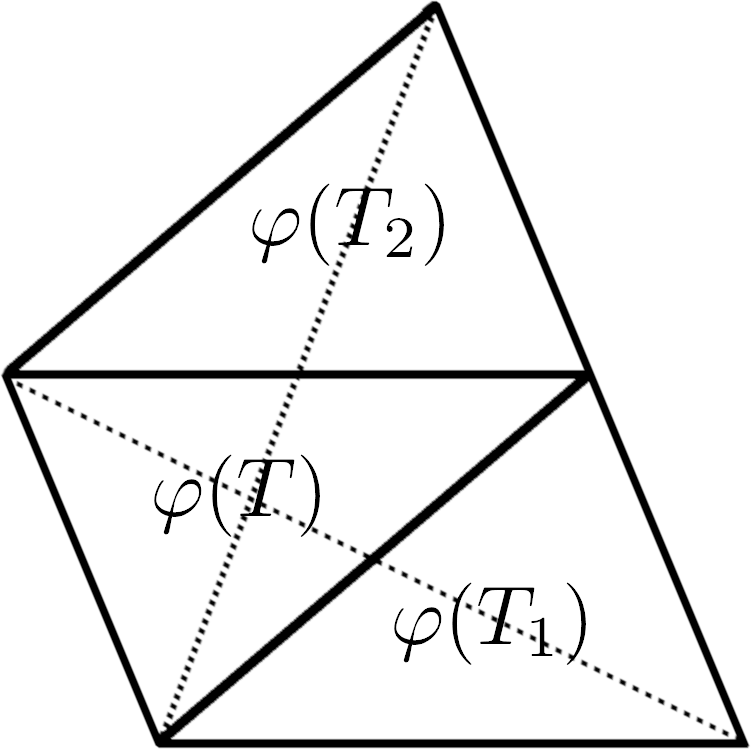
\includegraphics[width=.25\textwidth]{figs/spheretri_plane.png}
	\caption{The image under $\vphi$ of $T,T_1,T_2$.}
	\label{fig:sphtris_pl}
\end{figure}

Since $T\cup T_1$ and $T\cup T_2$ are both spherical quadrilaterals which overlap on the spherical triangle $T$, the images of $T\cup T_1$ and $T\cup T_2$ are Euclidean parallelograms of equal area which overlap on a shared triangle $\vphi(T)$.
	Therefore, the image of $T\cup T_1\cup T_2$ must 
	consist of two parallelograms, one of whose 
	edges is the diagonal of the other. In other words, 
	$\vphi(T\cup T_1\cup T_2)$ is a Euclidean trapezoid 
	whose boundary consists of four Euclidean geodesic 
	segments, as in \Cref{fig:sphtris_pl}.
	
	To find the contradiction, consider the point on the sphere at which $T$, $T_1$, and $T_2$ meet.  Since these triangles are all equilateral spherical triangles, the three angles at this point are each at least $\tfrac{\pi}{3}$ radians, because the sum of interior angles on a triangle is at least $\pi$.  Therefore, the total measure of the three angles at this point is at least $\pi$.  Therefore, the two geodesic segments which are part of the boundaries of $T_1$ and $T_2$ meet at this point at an angle of measure at least $\pi$, so together they do not form a geodesic.  Therefore, on the sphere, the region $T\cup T_1\cup T_2$ has a boundary consisting of five geodesic segments whereas its image has a boundary consisting of four, which contradicts the assumption that $\vphi$ and $\vphi^{-1}$ preserve geodesics.
\end{proof}


